\documentclass[aspectratio=169,9pt]{beamer}
\usepackage[french]{babel}
\selectlanguage{french}
\usepackage[utf8]{inputenc}
\usepackage{framed}

\makeatletter
\def\input@path{{../template_unisante/}}
\makeatother
\graphicspath{{../template_unisante/}{../template_unisante/logos/}{../images/}}
\usetheme{unisante}

\usepackage{tikz, tikz-cd}
\usepackage{pgf}
\usepackage{graphicx}
\usepackage[font=small,labelfont=bf]{caption}
\usepackage{subcaption}
\usepackage{hyperref}
\usepackage{multirow}
\usepackage{listings}
\usepackage{amsmath}
\usepackage{qrcode}
\usetikzlibrary{tikzmark,decorations.pathreplacing}

%%% Compact itemize, mirroring \compresslist from the poster %%%%%%%%%%%%%%%%%%%
\newcommand{\compresslist}{%
  \setlength{\itemsep}{2pt}%
  \setlength{\parskip}{0pt}%
  \setlength{\parsep}{0pt}%
}
\newcommand{\compressl}{%
  \setlength{\itemsep}{4pt}%
  \setlength{\parskip}{2pt}%
  \setlength{\parsep}{2pt}%
}
\definecolor{monvert}{rgb}{0.0, 0.5, 0.0}
\newcommand{\smallitem}[1]{{\fontsize{8pt}{9pt}\selectfont #1}}
\setbeamerfont{footnote mark}{size=\tiny}
\setbeamerfont{footnote}{size=\tiny}

\title[]{Caractérisation de la baisse des naissances en Suisse : analyse statistique de 2000 à 2025}
\author{Anthony Hauser, Julien Riou, Kaspar Staub}
\institute{\normalsize Unisanté}
\date{\normalsize Lausanne, 10 septembre 2026}

%% Contenu
\begin{document}
	
	
{
	\setbeamertemplate{footline}{} 
	\begin{frame}
		\titlepage
	\end{frame}
}
\addtocounter{framenumber}{-1}

\section*{Introduction}

%%% Background %%%%%%%%%%%%%%%%%%%%%%%%%%%%%%%%%%%%%%%%%%%%%%%%%%%%%%%%%%%%%%%%

\begin{frame}{La baisse de la fécondité en Suisse}
\begin{minipage}[t]{0.48\linewidth}
\textbf{Evolution 2000-2025}
\begin{itemize}\compresslist
\item \textbf{Indice conjoncturel de fécondité} (ICF) : nombre moyen d'enfants par femme
\item En Suisse, ICF de 1,29 en 2025 (au dessous du niveau de remplacement, 2.1 enfants par femme)
%COVID-19 : un \textbf{« pandemic roller-coaster »}, avec une baisse initiale, un rebond en 2021, puis une nouvelle baisse à partir de 2022.
\end{itemize}

\textbf{Raisons}
\begin{itemize}\compresslist
	\item \textbf{Structure par âge}: vieillissement de la population en âge de procréer.
	\item \textbf{Report de la parentalité}: les femmes ont des enfants plus tard (\emph{tempo effect}).
	\item Mais aussi une \textbf{réduction de la fécondité au cours de la vie} (\emph{quantum effect}) : les femmes ont moins d'enfants.\footnote[frame]{ Hellstrand et al., \emph{Demography} 2021;58(4):1373--1399.}
\end{itemize}

\vspace*{0.2cm}
\centering
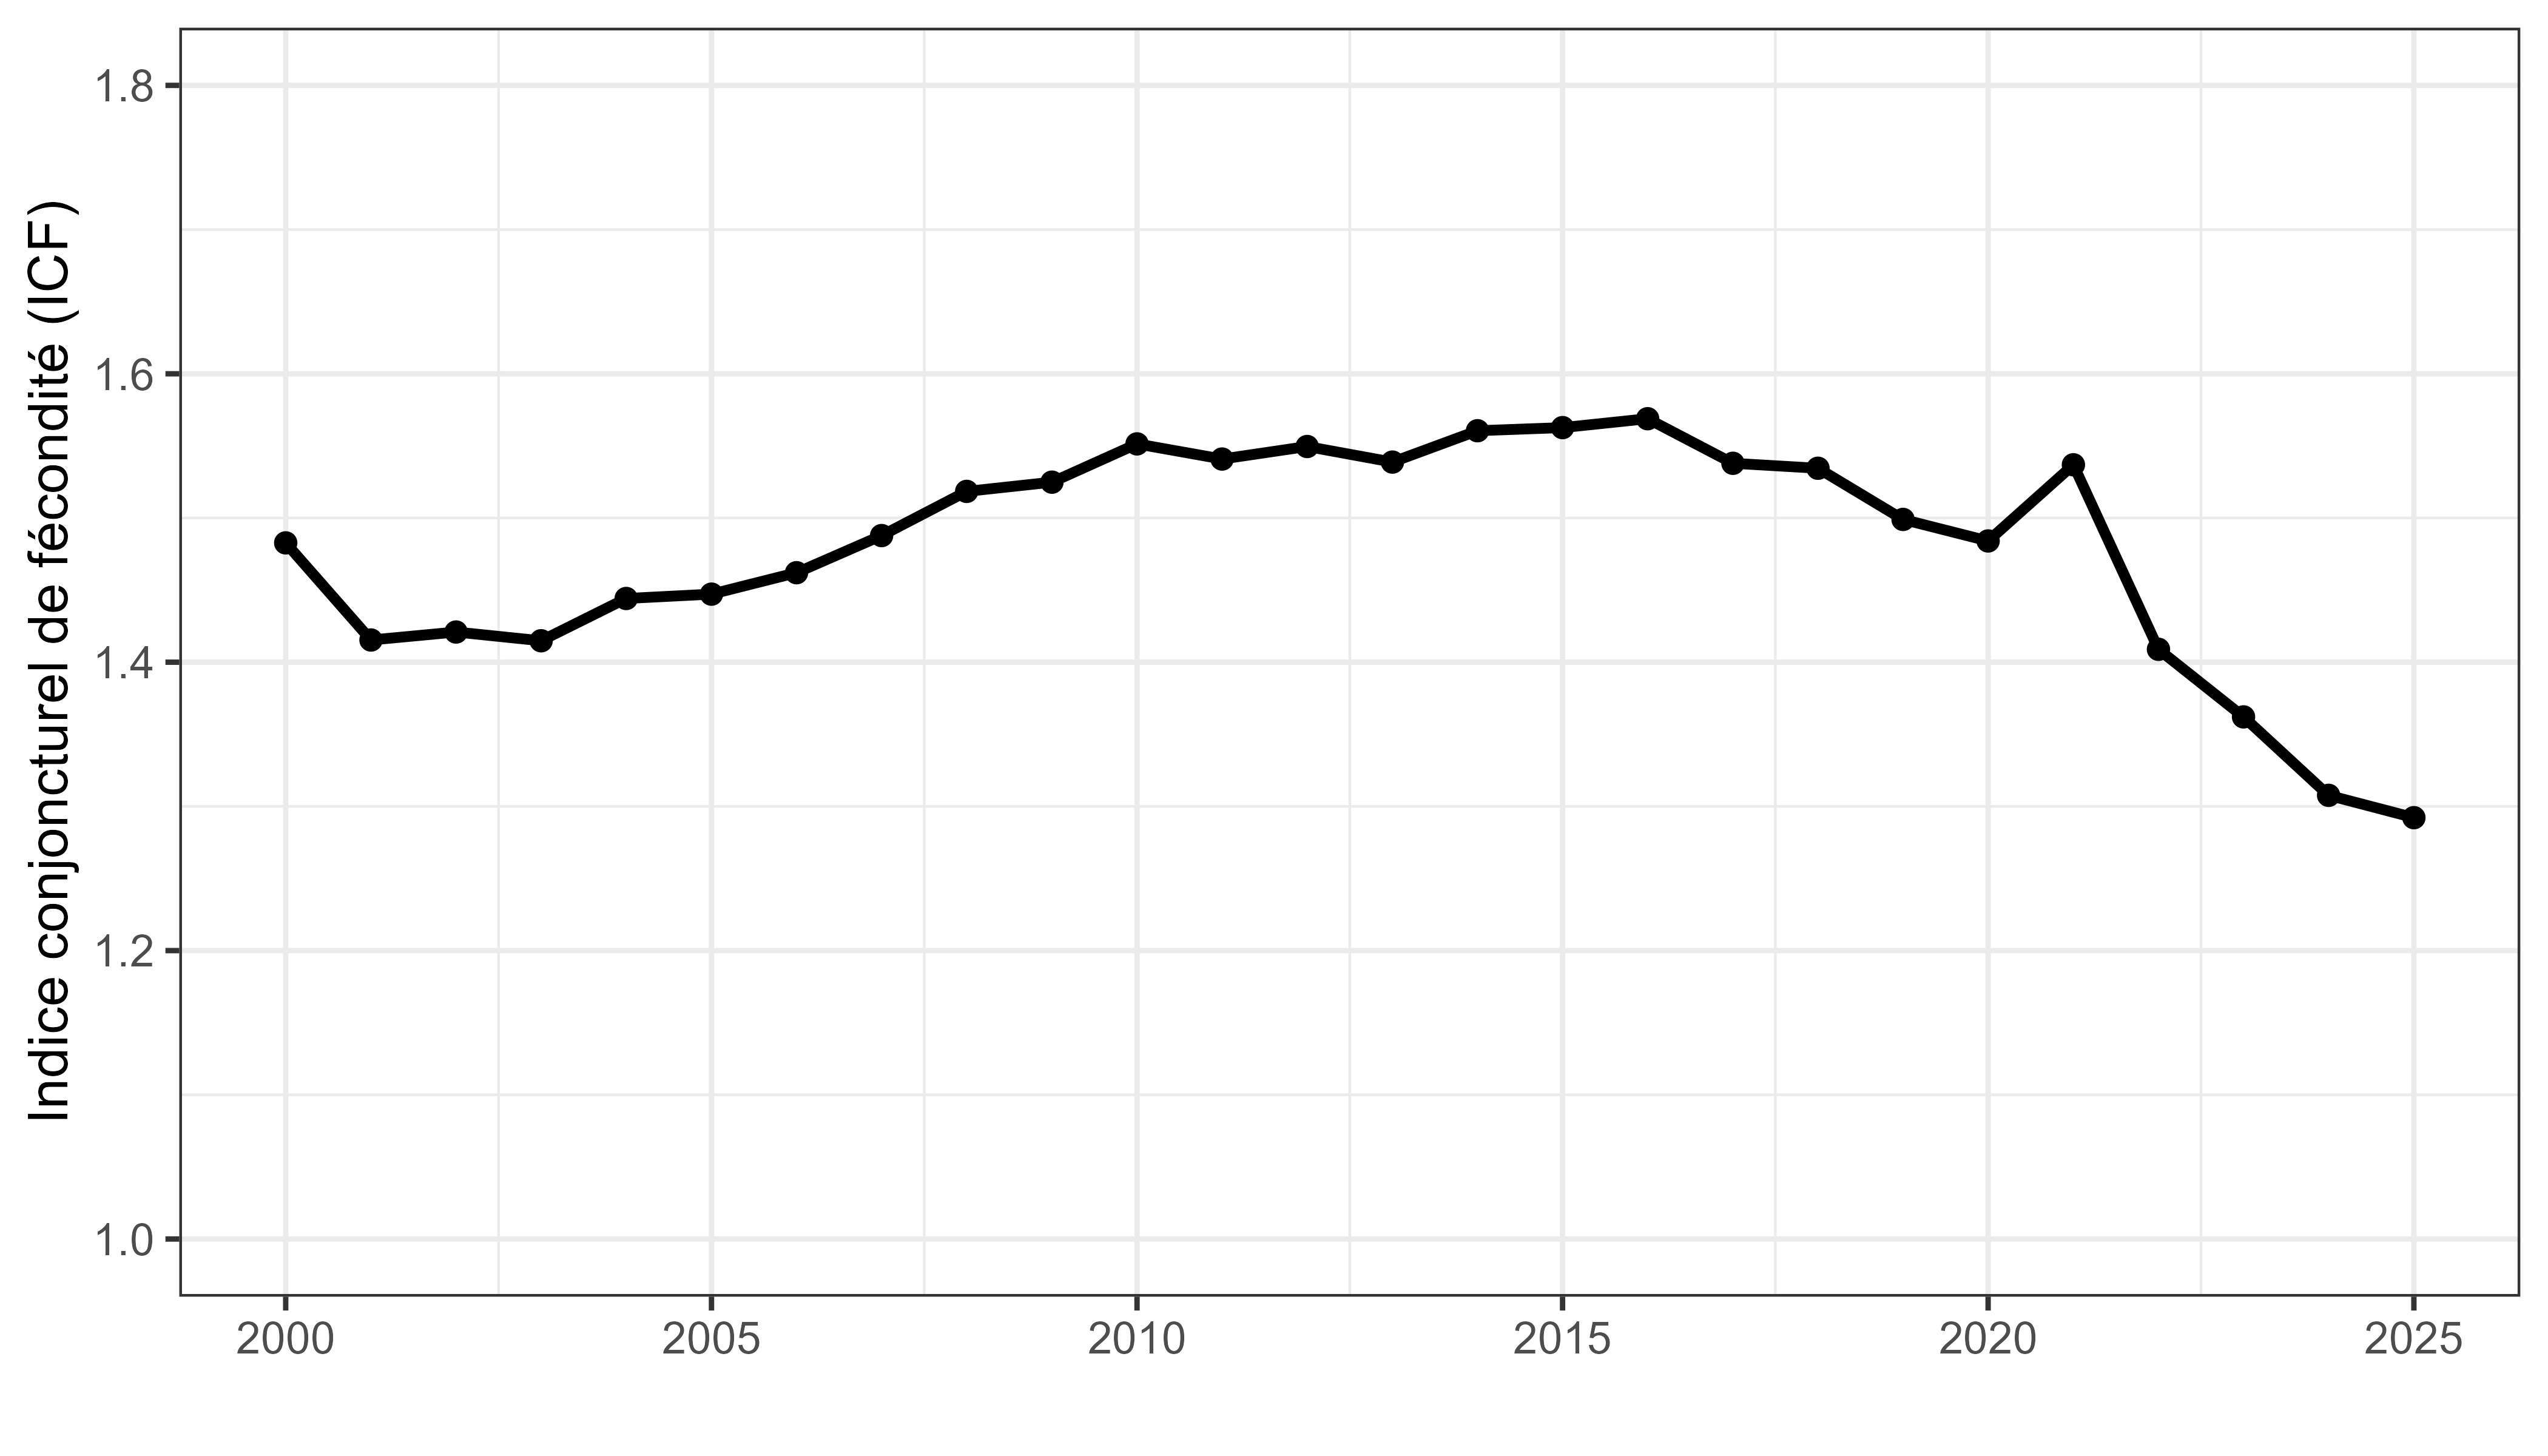
\includegraphics[width=0.8\linewidth,keepaspectratio]{icf_switzerland_2020_2025.png}
\end{minipage}
\hfill
\begin{minipage}[t]{0.48\linewidth}
\textbf{Comparaison historique}
\begin{itemize}\compresslist
\item Rebond observé en 2021 contraste avec les pandémies historiques (1889–90, 1918–20, 1957) \footnote[frame]{Matthes et al., \emph{Population Studies} 2025;79(3):463–478.}
\item Des phases de déclin déjà observées dans le passé.%On observe aussi que la phase de déclin observé actuellement n'a rien de nouveau.
\end{itemize}%permet de remettre en perspective
\vspace*{0.2cm}
\centering
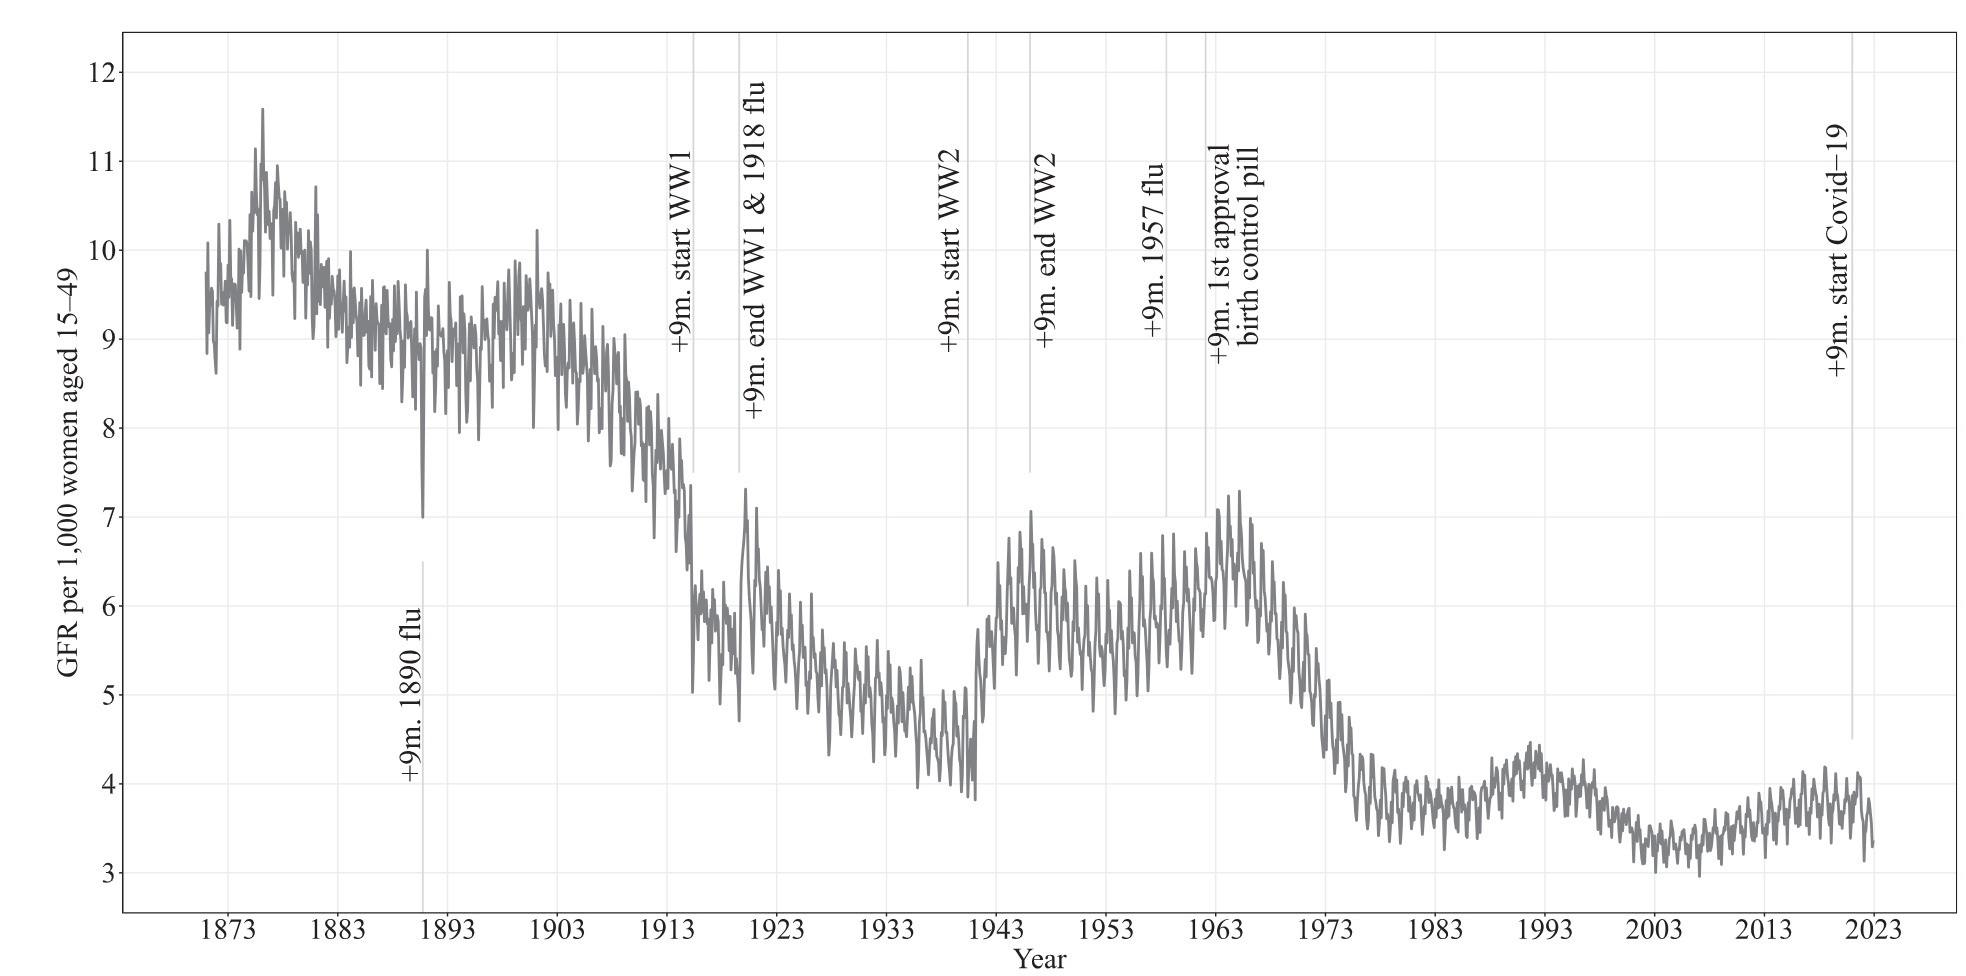
\includegraphics[width=1\linewidth,keepaspectratio]{matthes_historical_birth.png}
\end{minipage}
\end{frame}

\begin{frame}{Objectifs}

\begin{itemize}\compresslist
\item \textbf{Quantifier l’évolution de la natalité en Suisse (2000–2025)} en tenant compte de la structure de la population par âge et du report de la parentalité.

\item \textbf{Explorer les différences géographiques} de natalité et leurs déterminants.
\end{itemize}
\end{frame}



\begin{frame}{Modèle : calcul du déficit de naissance en 2000-2025}
	\begin{columns}[T]
		
		%%%%%%%%%%%%%%%%%%%%%%%%%%%%%%%%%%%%%%%%%%%%%%%%%%%%%%%%%%%%%%%%%%%%%%%%%
		% Colonne de gauche : données, excès/déficit, nombre attendu
		%%%%%%%%%%%%%%%%%%%%%%%%%%%%%%%%%%%%%%%%%%%%%%%%%%%%%%%%%%%%%%%%%%%%%%%%%
		\begin{column}{0.42\textwidth}
			\begin{itemize}\compresslist
				\item \textbf{Données} :
				\begin{itemize}\compresslist
					\item \textbf{Naissances} : données individuelles avec des informations sur la mère (age, muncipalité, nationalité, etc.)
					\item \textbf{Population} : nombre de femmes par âge et municipalité dans le temps
				\end{itemize}
				
				\item\textbf{Excès/déficit de naissance:} différence entre le nombre de naissances observé et attendu:\vspace{-0.1cm}
				$$E_{a}(t) = y_{a}(t) - \tilde{\mu}_{a}(t)$$ $$ E^r_{a}(t) = \dfrac{E_{a}(t)}{\tilde{\mu}_{a}(t)}$$
				
					\item Calcul du déficit de naissance au niveau:\\[0.1cm]
				\begin{minipage}[t]{4.2cm}   % largeur = un peu plus que la ligne la plus longue
					\vspace{-0.3cm}
					\begin{itemize}\compresslist
						\item national
						\item \tikzmark{a}communal
						\item \tikzmark{b}par sous-groupe (nationalité, parité)
					\end{itemize}
				\end{minipage}%
				\begin{tikzpicture}[overlay,remember picture]
					\draw[decorate,decoration={brace,amplitude=6pt}]   % sans mirror
					([xshift=2.6cm,yshift=1.6ex]pic cs:a) --
					([xshift=2.6cm,yshift=-2.8ex]pic cs:b)
					node[midway,right=6pt]{extrapolé};
				\end{tikzpicture}
				
			\end{itemize}
		\end{column}
		
		%%%%%%%%%%%%%%%%%%%%%%%%%%%%%%%%%%%%%%%%%%%%%%%%%%%%%%%%%%%%%%%%%%%%%%%%%
		% Colonne de droite : modèle bayésien
		%%%%%%%%%%%%%%%%%%%%%%%%%%%%%%%%%%%%%%%%%%%%%%%%%%%%%%%%%%%%%%%%%%%%%%%%%
		\begin{column}{0.58\textwidth}
			\begin{itemize}\compresslist
				\item \textbf{Nombre attendu de naissances :} \emph{nombre de naissances si le niveau de fécondité était resté constant lors des 25 dernières années.}\vspace{0.15cm}
				\begin{itemize}\compresslist
					\item Évolution du \textbf{nombre de femmes} en âge de procréer et de leur \textbf{structure par âge}
					\item \textbf{Report de la maternité} vers des âges plus élevés
					\item \textbf{Pas de tendance temporelle de la fécondité}
				\end{itemize}
				
				\item\textbf{Modèle bayésien:} Pour chaque âge $a$, on estime le nombre de naissance par mois:
				\vspace{0cm}
				$$y_{a}(t) \sim \text{Neg-Bin}\big(\mu_{a}(t),\phi\big)$$
				$$\log \mu_{a}(t) =  \textcolor{red}{f}(a+\textcolor{orange}{\theta(t)}) + \textcolor{blue}{\lambda_m(t)} +
				\textcolor{monvert}{\lambda_y(t)} +
				\log N_{a,t}$$
				\vspace{-0.2cm}
				\begin{itemize}\compresslist
					\item  \textcolor{red}{Fécondité par âge}: probabilité d'avoir un enfant pour une femme d'âge $a$.
					\item  \textcolor{orange}{Report de la maternité}
					\item \textbf{\textcolor{blue}{Effet aléatoire mensuel}}
					\item \textbf{\textcolor{monvert}{Effet aléatoire annuel}}: corrélation des naissances d'une certaine années
				\end{itemize}
			
			
			\end{itemize}
		\end{column}
		
	\end{columns}
\end{frame}

\begin{frame}{Calibration du modèle}
	texte:
	
	figure: fig1.png
\end{frame}

\begin{frame}{Déficit de naissances au niveau national}
	texte:
	
	figure: fig1.png	
\end{frame}

\begin{frame}{Déficit de naissances par commune}
	texte:
	
	figure: fig1.png	
\end{frame}

\begin{frame}{Résultats par sous-groupes: nationalité et parité}
	texte:
	
	figure: fig1.png
\end{frame}


\end{document}